% Standalone figure for the Statistical Mechanics notes.
% Build: pdflatex potentials.tex  (or run build.sh in this folder)
\documentclass[11pt,tikz,border=2pt]{standalone}
\usepackage{amsmath,amssymb}
\usetikzlibrary{arrows.meta, positioning}
\begin{document}
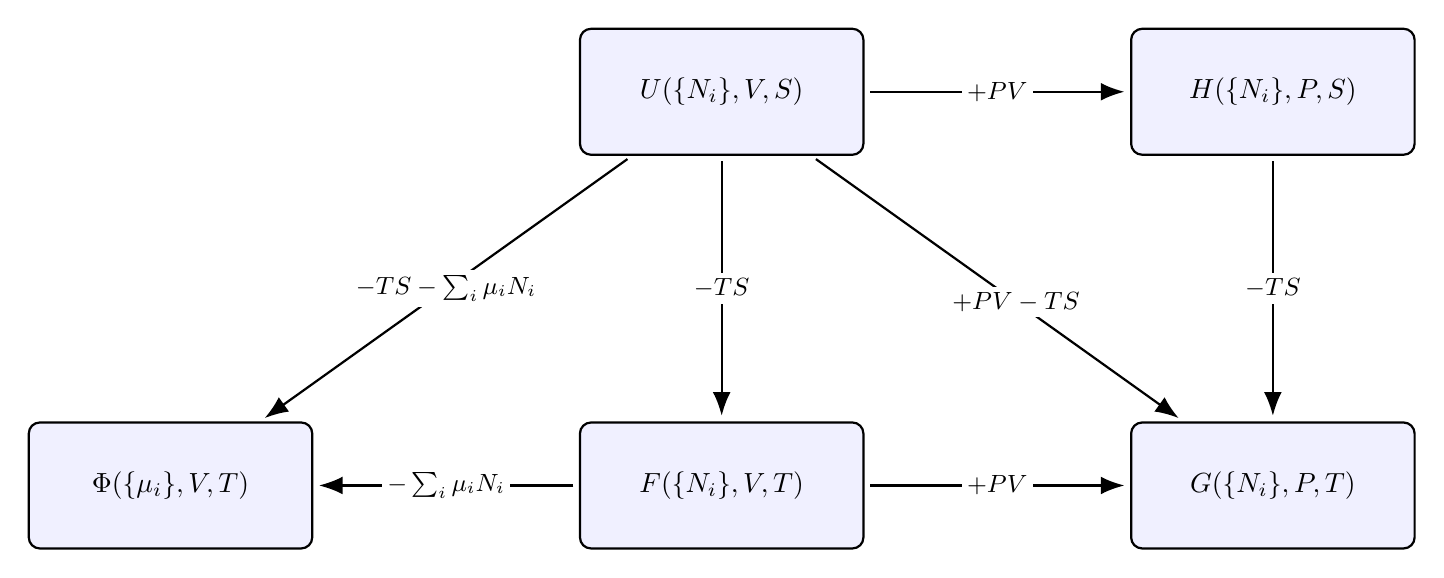
\begin{tikzpicture}[
    pot/.style={
        draw, rounded corners=4pt, thick,
        minimum width=3.6cm, minimum height=1.6cm,
        inner sep=4pt, align=center, fill=blue!6
    },
    arr/.style={-{Latex[length=3mm]}, thick, shorten >=2pt, shorten <=2pt},
    lbl/.style={fill=white, inner sep=2pt, font=\small}
]

% Nodes: U and F on the central axis, H/G on the right, Phi mirrored on the left
\node[pot] (U)   at (0,5)    {$U(\{N_i\},V,S)$};
\node[pot] (F)   at (0,0)    {$F(\{N_i\},V,T)$};
\node[pot] (H)   at (7,5)    {$H(\{N_i\},P,S)$};
\node[pot] (G)   at (7,0)    {$G(\{N_i\},P,T)$};
\node[pot] (Phi) at (-7,0)   {$\Phi(\{\mu_i\},V,T)$};

% Right-hand square
\draw[arr] (U) -- node[lbl] {$+PV$} (H);
\draw[arr] (U) -- node[lbl] {$-TS$} (F);
\draw[arr] (H) -- node[lbl] {$-TS$} (G);
\draw[arr] (F) -- node[lbl] {$+PV$} (G);
\draw[arr] (U) -- node[lbl, pos=0.55] {$+PV-TS$} (G);

% Left-hand (mirrored) edges
\draw[arr] (F) -- node[lbl] {$-\sum_i \mu_i N_i$} (Phi);
\draw[arr] (U) -- node[lbl, pos=0.5] {$-TS-\sum_i \mu_i N_i$} (Phi);

\end{tikzpicture}
\end{document}
